\section{Results}

\subsection{Semantic Segmentation}
EoMT-Cityscapes is the best model with 81.68\% mIoU among the compared model. Beside them ERFNet (72.50\%) is competitive for a pixel-based model.

\begin{table}[!htbp]
\centering
\small
\caption{Selected per-class IoU (\%) on \texttt{Cityscapes val}. EoMT-COCO scores 0\% on classes with no COCO equivalent.}
\label{tab:perclass}
\begin{tabular}{lcc}
\toprule
Class & EoMT-COCO & EoMT-Cityscapes \\
\midrule
pole          & \textbf{0.00}  & 71.04 \\
rider         & \textbf{0.00}  & 71.11 \\
traffic sign  & \textbf{4.74}  & 82.13 \\
\midrule
road          & 94.13 & 98.40 \\
car           & 84.33 & 95.54 \\
bicycle       & 73.34 & 81.27 \\
\midrule
\textbf{Mean} & \textbf{55.17} & \textbf{81.68} \\
\bottomrule
\end{tabular}
\end{table}

EoMT-COCO scores 0\% IoU on \texttt{pole, rider}, and near-0\% on \texttt{traffic sign} (Table~\ref{tab:perclass}) because COCO has no equivalent label.
It is not the problem of the model but a label space mismatch. It is the motivation for fine-tuning.
Fine-tuning lifts mIoU from 55.17 to 78.85, recovers the most of the gap. This result shows that COCO's DINOv2-backed visual priors work well, the only problem was the classification head, not the features.

\subsection{Anomaly Segmentation}

\paragraph{Pixel-based vs mask-based.}

We see these results from the comparison of ERFNet and EoMT (Table~\ref{tab:temperature_combined}):
\begin{itemize}
    \item On RoadAnomaly-21 dataset, ERFNet's MaxLogit is 38.31, and EoMT-Cityscapes' MaxEntropy is 77.88. There is a 40\% point difference
    \item On RoadObstacle-21 dataset, ERFNet's MaxLogit is 4.63 and EoMT-Cityscapes' MSP is 90.11. There is a 85\% point difference
    \item On RoadAnomaly dataset, ERFNet's MaxLogit 15.58 and EoMT-Cityscapes' MaxEntropy 78.14. There is a 63\% point difference
\end{itemize}
With these results, we find that on most benchmarks, the EoMT's models substantially outperform the ERFNet. Mask-based classification 
creates smooth shapes because it looks at the whole object at once. However, pixel-softmax looks at each pixel one by one, that's why it is vulnerable to noise.

\paragraph{Effect of fine-tuning.}

To see the effect of the fine-tuning, we compare the EoMT-Cityscapes with EoMT-Fine-tuned on AuPRC (Table~\ref{tab:temperature_combined}).
\begin{itemize}
    \item On RoadAnomaly-21 dataset: MSP score drops from 74.36\% to 57.15\% (~17\% change)
    \item On RoadObstacle-21 dataset: MSP score drops from 90.11\% to 73.61\% (~16\% change)
    \item On RoadAnomaly dataset: MSP score drops from 75.69\% to 54.99\% (~21\% change)
    \item On FS L\&F dataset: MSP score increases from 25.42\% to 27.11\% (~2\% change)
\end{itemize}
According to these results, EoMT-Fine-tuned recovers closed set mIoU (Table~\ref{tab:temperature_combined}) but decrease the anomaly scores compared to training from scratch on Cityscapes.
This happens because training the model for a short time makes it hyper-focused on normal objects, and this ruins its ability to spot unusual things. 

\begin{figure}[!htbp]
\centering
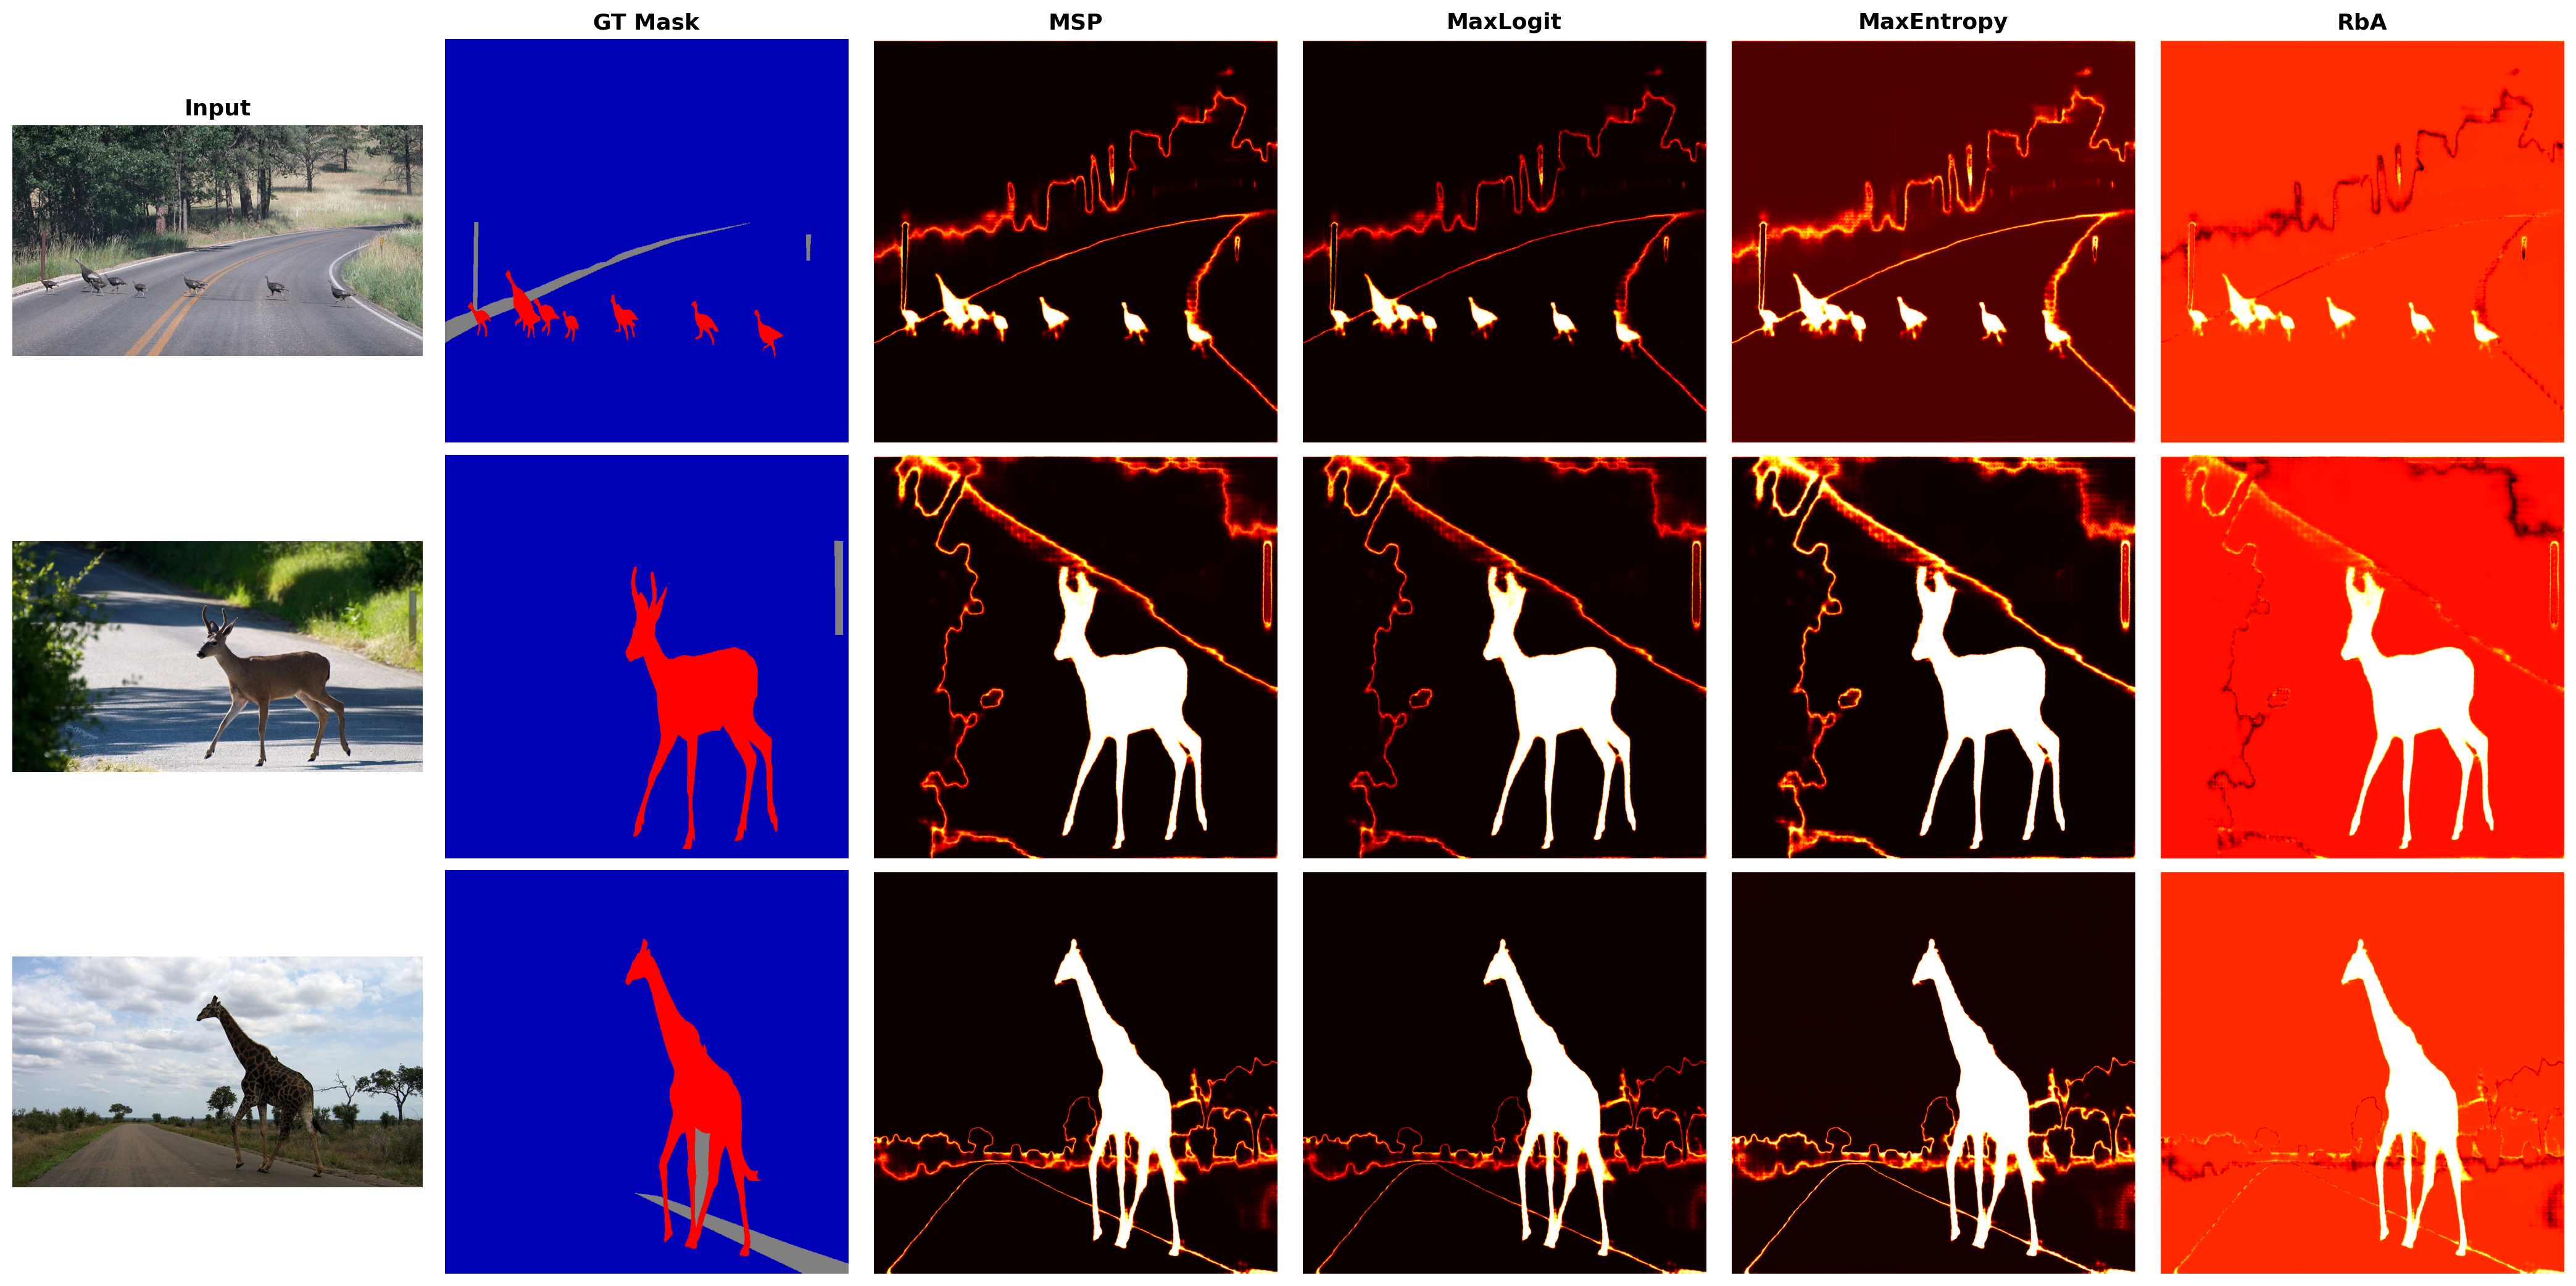
\includegraphics[width=\linewidth]{results/figures/step8/step8_anomaly_maps.png}
\caption{Qualitative comparison of anomaly score maps on RoadAnomaly21. 
Each row shows an input image alongside score maps produced by MSP, MaxLogit, 
MaxEntropy, and RbA for EoMT-Cityscapes.}
\label{fig:step8}
\end{figure}
\paragraph{Comparison of scoring functions.}
Interesting finding here is that MaxLogit beats MSP and MaxEntropy on ERFNet (38.31 vs 29.09 vs 30.96 on RA-21), but on EoMT they are almost same.
This result shows that scoring-method choice depends on the architecture.

\begin{table*}[!tp]
\centering
\caption{Temperature scaling results across the three models. Only $T \in \{0.5, 1.0, 2.0\}$ shown; intermediate values $T \in \{0.75, 1.1, 1.5\}$ follow the same trend. AuPRC ($\uparrow$, \%) and FPR95 ($\downarrow$, \%) on five benchmarks. RbA is omitted for ERFNet as it is incompatible with pixel-based architectures.}
\label{tab:temperature_combined}
\resizebox{\textwidth}{!}{
\begin{tabular}{llc|cc|cc|cc|cc|cc}
\toprule
 & & \multicolumn{2}{c|}{RA-21} & \multicolumn{2}{c|}{RO-21} & \multicolumn{2}{c|}{FS L\&F} & \multicolumn{2}{c|}{FS Static} & \multicolumn{2}{c}{RoadAnom} \\
Model & Method & $T$ & AuPRC$\uparrow$ & FPR95$\downarrow$ & AuPRC$\uparrow$ & FPR95$\downarrow$ & AuPRC$\uparrow$ & FPR95$\downarrow$ & AuPRC$\uparrow$ & FPR95$\downarrow$ & AuPRC$\uparrow$ & FPR95$\downarrow$ \\
\midrule
ERFNet & MSP & 0.5 & 27.05 & 62.75 & 2.42 & 63.24 & 1.28 & 66.73 & 6.6 & 43.48 & 12.19 & 82.04 \\
 &  & 1.0 & 29.09 & 62.57 & 2.71 & 65.27 & 1.75 & 50.62 & 7.47 & 41.84 & 12.42 & 82.59 \\
 &  & 2.0 & 30.6 & 65.05 & 3.0 & 72.74 & 2.69 & 47.92 & 9.54 & 41.29 & 12.64 & 84.58 \\
 & MaxEntropy & 0.5 & 28.58 & 62.74 & 2.64 & 63.73 & 1.59 & 52.82 & 7.04 & 43.2 & 12.33 & 82.26 \\
 &  & 1.0 & 30.96 & 62.67 & 3.04 & 65.95 & 2.58 & 50.19 & 8.84 & 41.55 & 12.67 & 82.76 \\
 &  & 2.0 & 30.27 & 67.09 & 2.97 & 75.98 & 3.51 & 47.1 & 11.72 & 41.75 & 12.79 & 85.6 \\
\midrule
EoMT-Cityscapes & MSP & 0.5 & 74.21 & 33.73 & 90.1 & 0.55 & 25.4 & 14.91 & 54.33 & 34.94 & 75.51 & 19.37 \\
 &  & 1.0 & 74.36 & 33.73 & 90.11 & 0.55 & 25.42 & 14.9 & 54.35 & 34.94 & 75.69 & 19.31 \\
 &  & 2.0 & 74.55 & 33.73 & 90.11 & 0.55 & 25.44 & 14.9 & 54.36 & 34.93 & 75.87 & 19.28 \\
 & MaxEntropy & 0.5 & 77.43 & 33.68 & 90.09 & 0.59 & 29.55 & 14.83 & 53.21 & 34.91 & 78.43 & 19.03 \\
 &  & 1.0 & 77.88 & 33.6 & 90.01 & 0.68 & 29.56 & 14.72 & 52.51 & 34.84 & 78.14 & 18.79 \\
 &  & 2.0 & 77.91 & 33.53 & 89.97 & 0.72 & 29.01 & 14.65 & 51.46 & 34.77 & 77.43 & 18.63 \\
 & RbA & 0.5 & 69.57 & 76.02 & 73.77 & 99.95 & 26.0 & 67.27 & 55.85 & 84.55 & 74.12 & 44.02 \\
 &  & 1.0 & 69.99 & 80.06 & 86.97 & 99.95 & 25.97 & 8.79 & 56.11 & 82.68 & 74.62 & 20.41 \\
 &  & 2.0 & 70.83 & 91.98 & 88.25 & 99.94 & 25.92 & 10.05 & 55.91 & 35.88 & 75.09 & 17.96 \\
\midrule
EoMT-Fine-tuned & MSP & 0.5 & 58.59 & 98.6 & 73.69 & 25.1 & 27.07 & 26.22 & 53.35 & 39.78 & 54.96 & 16.27 \\
 &  & 1.0 & 57.15 & 98.61 & 73.61 & 25.09 & 27.11 & 26.16 & 53.41 & 39.74 & 54.99 & 16.22 \\
 &  & 2.0 & 56.61 & 98.62 & 73.57 & 25.09 & 27.13 & 26.15 & 53.43 & 39.72 & 55.0 & 16.2 \\
 & MaxEntropy & 0.5 & 54.1 & 98.71 & 73.43 & 28.83 & 27.91 & 26.21 & 53.87 & 39.53 & 55.83 & 15.28 \\
 &  & 1.0 & 54.49 & 98.82 & 72.62 & 57.49 & 28.56 & 26.33 & 54.27 & 39.25 & 56.22 & 14.78 \\
 &  & 2.0 & 54.65 & 98.82 & 71.69 & 60.82 & 29.18 & 26.24 & 54.5 & 38.76 & 56.33 & 14.51 \\
 & RbA & 0.5 & 51.52 & 99.53 & 62.1 & 99.98 & 31.42 & 78.97 & 56.29 & 89.51 & 52.39 & 81.57 \\
 &  & 1.0 & 51.82 & 99.85 & 64.22 & 99.98 & 30.61 & 26.92 & 56.29 & 90.34 & 56.14 & 13.38 \\
 &  & 2.0 & 51.88 & 99.87 & 66.12 & 99.98 & 30.36 & 24.49 & 55.73 & 89.65 & 56.57 & 12.09 \\
\bottomrule
\end{tabular}}
\end{table*}

RbA has a different pattern in here. It achieves highest AuPRC on FS L\&F (30.61) and FS Static (56.29) for EoMT-Fine-tuned. 
However, it also produces high score for FPR95, so it separates the outlier but it is too sensitive so it makes a lot of false alarms.  


%\paragraph{Qualitative results.}
%Figure~\ref{fig:step8} shows anomaly score maps for the four scoring methods on representative RoadAnomaly21 images.

\subsection{Temperature Scaling Study}

For temperature scaling, we tried $T \in \{0.5, 0.75, 1.0, 1.1, 1.5, 2.0\}$ on MSP, MaxEntropy, and RbA 
for EoMT-Cityscapes, EoMT-Fine-tuned, and ERFNet.
Main finding that AuPRC is mostly stable across $T$ (Table~\ref{tab:temperature_combined}).
\begin{itemize}
    \item In EoMT-Cityscapes (Table~\ref{tab:temperature_combined}), MSP AuPRC on RA-21 stays in a 0.3\% window, and MaxEntropy stays in a 0.5\% window.
    \item In EoMT-Fine-tuned (Table~\ref{tab:temperature_combined}), It follows similar pattern as EoMT-Cityscapes
    \item In ERFNet (Table~\ref{tab:temperature_combined}), MSP on RA-21 has a change range for 3\%, but its AuPRC is so low that the gain is not meaningful. 
\end{itemize}

Interesting finding that RbA's AuPRC is stable, but its FPR95 swings with T:
\begin{itemize}
    \item EoMT-Cityscapes RbA on FS L\&F: FPR95=67.27 at T=0.5 vs 8.79 at T=1.0
    \item EoMT-Cityscapes RbA on RoadAnomaly: FPR95's score decreases from 20.41 at T=1.0 to 17.96 at T=2.0.
    \item EoMT-Fine-tuned RbA on RoadAnomaly: FPR95 = 81.57 at T=0.5 vs 12.09 at T=2.0
\end{itemize}

As result, we found that T=1.0 is competitive for AuPRC most settings. Temperature scaling doesn't meaningfully improve AuPRC, and can shift the FPR95 results, especially for RbA, but it is not a consistent gain.
Post-hoc temperature calibration is not a reliable method for improving anomaly segmentation on these benchmarks.